% Luebeck-default-default: buen outline arriba, lindos numeros/itemize, feo que se ve abajo el autor
% ilmenau: como Darmstadt pero más ordenado arriba y más feo
% Darmstadt: bueno pero son feos los itemize

\documentclass[
%aspectratio=169,
aspectratio=43,
hyperref={pdfpagelabels=false},
x  color={tables}]{beamer}



\usepackage[utf8]{inputenc}
\usepackage[T1]{fontenc}
\usepackage[english,spanish]{babel}

\usepackage{inconsolata}

\usepackage{tikz}
\usetikzlibrary{shapes.arrows,shapes,decorations,positioning,matrix,chains,decorations.pathreplacing,arrows}

\usepackage{listings}
\usepackage[numbered,framed]{matlab-prettifier}
\usepackage{color} %red, green, blue, yellow, cyan, magenta, black, white
\definecolor{mygreen}{RGB}{28,172,0} % color values Red, Green, Blue
\definecolor{mylilas}{RGB}{170,55,241}

\usepackage{pgffor}
\usepackage{pgfplots}
\pgfplotsset{
compat=1.6,
every axis/.append style={font=\small}  
}

\usepackage{tabulary}
%\usepackage[table]{xcolor}
\usepackage{colortbl}

\usepackage{amssymb}
\usepackage{lmodern}

\usetheme{Boadilla}
\usecolortheme{dolphin}
\setbeamertemplate{footline}[frame number]


\useinnertheme{rectangles} % rectangles for itemize and enumerate

\beamertemplatenavigationsymbolsempty 

%\unaccentedoperators
\usefonttheme{professionalfonts}
% Absolute positioning
%\usepackage[absolute,overlay]{textpos}
%  \setlength{\TPHorizModule}{1mm}
%  \setlength{\TPVertModule}{1mm}

% usage:  \begin{textblock}{*width*}(*x-position,y-position*)
%\begin{textblock}{20}(40,20)
%      \includegraphics{file}
%    \end{textblock}


% abs pos with tikz
%\begin{tikzpicture}[remember picture,overlay]
%  \node[anchor=south west,inner sep=0pt] at ($(current page.south west)+(2cm,5cm)$) {
%     \includegraphics{imgfile}
%  };
%\end{tikzpicture}
%\lstset{language=Matlab,%
%    %basicstyle=\color{red},
%    breaklines=true,%
%    morekeywords={matlab2tikz},
%    keywordstyle=\color{blue},%
%    morekeywords=[2]{1}, keywordstyle=[2]{\color{black}},
%    identifierstyle=\color{black},%
%    stringstyle=\color{mylilas},
%    commentstyle=\color{mygreen},%
%    showstringspaces=false,%without this there will be a symbol in the places where there is a space
%    numbers=left,%
%    numberstyle={\tiny \color{black}},% size of the numbers
%    numbersep=9pt, % this defines how far the numbers are from the text
%    emph=[1]{for,end,break},emphstyle=[1]\color{red}, %some words to emphasise
%    %emph=[2]{word1,word2}, emphstyle=[2]{style},    
%}

\lstset{
  style              = Matlab-editor,
  basicstyle         = \ttfamily,
  escapechar         = ",
  mlshowsectionrules = true,
}



\title{
    {\Huge FFT}    
}
  

\author{
    {\large  }\\
}

\date{}

%\titlegraphic{
%
%    \includegraphics[width=2cm]{img/logounlp}\\
%            {\large Universidad Nacional de La Plata} 
%}



\newcolumntype{L}[1]{>{\raggedright\let\newline\\\arraybackslash\hspace{0pt}}m{#1}}
\newcolumntype{C}[1]{>{\centering\let\newline\\\arraybackslash\hspace{0pt}}m{#1}}
\newcolumntype{R}[1]{>{\raggedleft\let\newline\\\arraybackslash\hspace{0pt}}m{#1}}

\DeclareMathOperator*{\Max}{Maximizar}

\newcommand{\twocols}[3][0.5]{
\begin{columns}
\begin{column}{#1\textwidth}
#2
\end{column}

\begin{column}{#1\textwidth}  
#3
\end{column}

\end{columns}
}


%\newcommand{\twobytwographics}[12]{
%
%\begin{tabular}{|c|c|}
%\includegraphics[scale=#1]{#2} & \includegraphics[scale=#4]{#5} \\
%#3 &  #6\\
%\includegraphics[scale=#7]{#8} & \includegraphics[scale=#10]{#11}\\
%#9 &  #12
%}


\newcommand{\twographics}[4]{
\twocols{\includegraphics[scale=#1]{#2}}{\includegraphics[scale=#3]{#4}}
}


\newcommand{\gesturemodel}[3]{
\centering #1 \vspace{5pt}
  \twocols[0.35]{
    \frame{ \includegraphics[scale=0.75]{features/#2}}
  }{
        \centering
    \frame{\includegraphics[scale=0.75]{features/#3}} 
  }
}




\newenvironment{myframe}{\begin{frame}  
%\vspace{-5.9pt} 
}{\end{frame}}

\newenvironment<>{varblock}[2][\textwidth]{
    \begin{center}
      \begin{minipage}{#1}
        \setlength{\textwidth}{#1}
          \begin{actionenv}#3
            \def\insertblocktitle{#2}
            \par
            \usebeamertemplate{block begin}}
  {\par
      \usebeamertemplate{block end}
    \end{actionenv}
  \end{minipage}
\end{center}}



\newcommand{\blockitemize}[2]{
\begin{block}{#1}
\centering
\begin{itemize}
#2
\end{itemize}
\end{block}
}


\def\mytemparray{}

%
\newcommand\abspos[3]{%
    \bgroup
    \def\mytemparray{{ #2 }}
    \pgfmathparse{\mytemparray[0]} \edef\mya{\pgfmathresult}
    \pgfmathparse{\mytemparray[1]} \edef\myb{\pgfmathresult}
    \pgfmathparse{\mytemparray[2]} \edef\myc{\pgfmathresult} %also possible \pgfmathsetmacro
    \begin{tikzpicture}[remember picture, overlay]
            \node[anchor=#1, opacity=\myc] at ( \mya pt, \myb  pt) {#3};
    \end{tikzpicture}%
        %
    %
    \egroup
%
}

%  \rowcolors{1}{gray!15}{gray!15}

\newcommand{\cellcolorgraphictoc}{\cellcolor{blue!40}}

\newcommand{\graphictocresults}{
\begin{tabular}{C{0.5\linewidth}C{0.5\linewidth}}
 \includegraphics[scale=0.35]{intro/work/hand_db} & \includegraphics[scale=0.2]{intro/work/representaciones}\\
[-1.5ex] Base de datos de gestos  & Modelo y representaciones de gestos \\
\includegraphics[scale=0.2]{intro/work/cnc} & \includegraphics[width=0.34\textwidth]{results/defense_cnc_n} \cellcolorgraphictoc\\  
[-1.5ex] Clasificador Neuronal Competitivo (CNC) & Resultados \cellcolorgraphictoc
\end{tabular}
}

\newcommand{\graphictocdb}{
\begin{tabular}{C{0.5\linewidth}C{0.5\linewidth}}
\cellcolorgraphictoc 

 \includegraphics[scale=0.35]{intro/work/hand_db} \cellcolorgraphictoc & \includegraphics[scale=0.2]{intro/work/representaciones} \cellcolorgraphictoc\\
[-1.5ex] Base de datos de gestos \cellcolorgraphictoc & Modelo y representaciones de gestos \cellcolorgraphictoc \\
\includegraphics[scale=0.2]{intro/work/cnc} & \includegraphics[width=0.34\textwidth]{results/defense_cnc_n} \\  
[-1.5ex] Clasificador Neuronal Competitivo (CNC) & Resultados
\end{tabular}
}

\newcommand{\graphictoccnc}{
  \begin{tabular}{C{0.5\linewidth}C{0.5\linewidth}}
 \includegraphics[scale=0.35]{intro/work/hand_db} & \includegraphics[scale=0.2]{intro/work/representaciones}\\
  [-1.5ex] Base de datos de gestos  & Modelo y representaciones de gestos \\
  \includegraphics[scale=0.2]{intro/work/cnc} \cellcolorgraphictoc & \includegraphics[width=0.34\textwidth]{results/defense_cnc_n} \\  
  [-1.5ex] Clasificador Neuronal Competitivo (CNC) \cellcolorgraphictoc & Resultados
  \end{tabular}
}



\newcommand{\wv}{\ve{w}}
\newcommand{\cc}{$\ve{cc}$}
\newcommand{\ve}[1]{\mathbf{#1} }
\newcommand{\derivative}[2]{\dv{#1}{#2}}
\newcommand{\dv}[2]{\frac{\partial #1}{\partial #2}}

%\newcommand{\defsetsimple}[1]{ \{ #1 \} }
%\newcommand{\defset}[2]{ \{ #1 \; \mid \; #2  \} }

%drawing



% AXIS

\newcommand{\correctaxiscenter}{
\pgfplotsset{
    standard/.style={
        axis x line=middle,
        axis y line=middle,
        enlarge x limits=0.15,
        enlarge y limits=0.15,
        every axis x label/.style={at={(current axis.right of origin)},anchor=north west},
        every axis y label/.style={at={(current axis.above origin)},anchor=north east}
    }
}
}

\newcommand{\axishundred}{xmin=-100,xmax=100,ymin=-100,ymax=100}
\newcommand{\axisten}{xmin=-10,xmax=10,ymin=-10,ymax=10}
\newcommand{\axisunit}{xmin=-1,xmax=1,ymin=-1,ymax=1}
\newcommand{\axissquare}[1]{xmin=-#1,xmax=#1,ymin=-#1,ymax=#1}
\newcommand{\axisrectangular}[2]{xmin=-#1,xmax=#1,ymin=-#2,ymax=#2}


\newcommand{\drawaxiss}[1]{
\draw [<->] (-#1,0) -- (#1,0);
\draw [<->] (0,-#1) -- (0,#1);
}

\newcommand{\myaxis}[2][]{
\begin{axis}[#1,anchor=origin, x=1cm, y=1cm]  % Align the origins
#2    
\end{axis}
}
\newcommand{\rectangularaxis}[4][]{
\myaxis[\axisrectangular{#3}{#4},#1]{#2}
}


\newcommand{\squareaxis}[3][]{
\myaxis[\axissquare{#3},#1]{#2}
}

\newcommand{\standardaxis}[2][]{
\myaxis[\axisten,#1]{#2}
}

\newcommand{\configureDiscard}{}

\newcommand{\resultsaxis}[3][]{
\correctaxiscenter
\configureDiscard

\pgfplotsset{
%    every axis/.append style={font=\small}  
}

\myaxis[legend pos=south east, every node near coord/.append style={font=\huge},ylabel=cc,xlabel=#3,#1,ytick={0,25,50,75,100}]{#2}
}

\newcommand{\addplotresults}[6]{
\addplot+[selecting={#1}{#2},#6] table[x index=#3, y index=#4,col sep=comma] {datos/#5};
\addlegendentry{$#1 = {#2}$};
}


%GAUSSIAN

\pgfmathdeclarefunction{invgauss}{2}{%
  \pgfmathparse{sqrt(-2*ln(#1))*cos(deg(2*pi*#2))}%
}
\newcommand{\addplotgaussian}[3]{
\addplot [only marks, samples=#1] ({invgauss(rnd,rnd)+#2},{invgauss(rnd,rnd)}+#3);
}

\newcommand{\addgaussianscatter}[4][30]{
\addplot [only marks, mark=#2,samples=#1] ({invgauss(rnd,rnd)+#3},{invgauss(rnd,rnd)+#4});
}


%aprendizaje

%areas


\newcommand{\classcircle}[3]{\draw [ultra thick, fill={rgb:black,1;white,20}] (#1,#2) circle [radius=#3]
}

\newcommand{\classcirclename}[3]{\classcircle{#1}{#2}{4};
\node [above] at (#1,#2+4) {#3};
}


\newcommand{\classcirclenamelittle}[2]{
\classcircle{#1}{#2}{3.3};
}


\newcommand{\tresclases}{
\classcirclename{0}{4}{Clase 1};
\classcirclename{-5}{-4}{Clase 2};
\classcirclename{5}{-4}{Clase 3};
}


\newcommand{\tresclasessmall}{
\classcirclenamelittle{0}{2.5};
\classcirclenamelittle{-5}{-2.5};
\classcirclenamelittle{5}{-2.5};
}


%scatter plots

\newcommand{\simmetricgaussianscatter}[4][50]{
\addgaussianscatter[#1]{#2}{#3}{#4}
\addgaussianscatter[#1]{#2}{#3}{-#4}
\addgaussianscatter[#1]{#2}{-#3}{-#4}
\addgaussianscatter[#1]{#2}{-#3}{#4}
}


\newcommand{\datosclase}[5][50]{
\addgaussianscatter[#1]{#2}{#3}{#4}
%\addlegendentry{Clase #5};
}


\newcommand{\datostresclases}{
\datosclase{o}{0}{2.5}{1}
\datosclase{triangle}{-5}{-2.5}{2}
\datosclase{diamond}{5}{-2.5}{3}
}         

\newcommand{\datosdosclasessinpintar}{
\addgaussianscatter{o}{-5}{2}
\addgaussianscatter{o}{5}{-2}
}

\newcommand{\datosdosclases}{
\addgaussianscatterpositive{-5}{2}
\addgaussianscatternegative{5}{-2}
}

\newcommand{\datosdosclasesinvisible}{
\addgaussianscattermarkercolor{o}{black}{-5}{2}
\addgaussianscattermarkercolor{o}{black}{5}{-2}
}

\newcommand{\datosnoseparable}{
\addgaussianscatterpositive{5}{2}
\addgaussianscatterpositive{3}{4}
\addgaussianscatternegative{3}{5}
\addgaussianscatternegative{2}{6}
}

\newcommand{\datosdosclasescruzadas}{
\addgaussianscatterpositive{4}{4}
\addgaussianscatternegative{-4}{4}
\addgaussianscatternegative{4}{-4}
\addgaussianscatterpositive{-4}{-4}
}


\newcommand{\datosnolineal}{
\addgaussianscatterpositive{-5}{2}
\addgaussianscatterpositive{0}{3}
\addgaussianscatterpositive{-2}{3}
\addgaussianscatterpositive{-5}{-4}
\addgaussianscatterpositive{-4}{-1}

\addgaussianscatternegative{2.5}{-3}
\addgaussianscatternegative{5}{-2}
\addgaussianscatternegative{0}{-4}
\addgaussianscatternegative{1}{-3.2}
\addgaussianscatterpositive{4}{4}
}


\newcommand{\addgaussianscattermarkercolor}[5][30]{
\addplot [only marks, mark=#2,mark options={#3},samples=#1] ({invgauss(rnd,rnd)+#4},{invgauss(rnd,rnd)+#5});
}

\newcommand{\addgaussianscatterpositive}[2]{
\addgaussianscattermarkercolor{o}{positive}{#1}{#2}
}

\newcommand{\addgaussianscatternegative}[2]{
\addgaussianscattermarkercolor{o}{negative}{#1}{#2}
}


\newcommand{\addgaussianscattermarkercolort}[6][30]{
\addplot3[only marks, mark=#2,mark options={#3},samples=#1] ({invgauss(rnd,rnd)+#4},{invgauss(rnd,rnd)+#5},{invgauss(rnd,rnd)+#6});
}


\newcommand{\addgaussianscatterpositivet}[3]{
\addgaussianscattermarkercolort{o}{positive}{#1}{#2}{#3}
}

\newcommand{\addgaussianscatternegativet}[3]{
\addgaussianscattermarkercolort{o}{negative}{#1}{#2}{#3}
}


\newcommand{\datosdosclasesnolineal}{
\addgaussianscatterpositive{-5}{2}
\addgaussianscatterpositive{0}{3}
\addgaussianscatterpositive{-5}{-4}
\addgaussianscatterpositive{-4}{-1}
\addgaussianscatternegative{2.5}{-3}
\addgaussianscatternegative{5}{-1}
\addgaussianscatternegative{0}{-4}
\addgaussianscatternegative{1}{-3.2}
}

\newcommand{\classp}{oplus}
\newcommand{\classm}{halfcircle}


\newenvironment{neuralnetwork}{

\begin{tikzpicture}[
plain/.style={
  draw=none,
  fill=none,
  },
net/.style={
  matrix of nodes,
  nodes={
    draw,
    circle,
    inner sep=10pt
    },
  nodes in empty cells,
  column sep=2cm,
  row sep=4pt
  },
>=latex
]
}{
\end{tikzpicture}
}


\definecolor{pbblue}{HTML}{0A75A8}% filling color for the progress bar
\definecolor{pbgray}{HTML}{575757}% background color for the progress bar

%\newcommand{\nodedb}[1]{\node[set] (db) [#1] {Base de datos};}
\newcommand{\nodenewgesture}[1]{\node[set] (newgesture) [#1] {Nuevo gesto};}
\newcommand{\nodetraining}[1]{  \node[function] (training) [#1] {Entrenamiento} ;}
\newcommand{\nodede}[1]{\node[setd] (de) [#1] {Conjunto de Entrenamiento};}
\newcommand{\nodedp}[1]{\node[setd] (dp) [#1] {Conjunto de Prueba};}
\newcommand{\nodemodel}[1]{\node[function] (model) [#1] {Modelo} ;}
\newcommand{\nodeinference}[1]{\node[inference] (inference) [#1] {Inferencia} ;}
\newcommand{\nodeclass}[1]{\node[inference] (class) [#1] {Clase} ;}
\newcommand{\nodeerror}[1]{\node[inference,minimum width=10em,minimum height=5em] (error) [#1] {Error} ;}
\newcommand{\nodepre}[1]{\node[setp] (pre) [#1] {Datos preprocesados};}
\newcommand{\nodeprenewgesture}[1]{\node[setp] (prenewgesture) [#1] {Nuevo gesto preprocesado};}
\newcommand{\nodefeature}[1]{\node[setp] (feature) [#1] {Representación Datos};}
\newcommand{\nodefeaturenewgesture}[1]{\node[setp] (featurenewgesture) [#1] {Representación nuevo gesto};}

%\newcommand{\node}[1]{}

\newcommand{\tikzstylesbig}{
\tikzset{
node distance=5cm,
set/.style={circle,text width=3cm,align=center,fill=green!50,font=\sffamily\Large},
setd/.style={circle,text width=3cm,align=center,fill=green!30,font=\sffamily\Large},
setp/.style={circle,text width=3cm,align=center,fill=green!20,font=\sffamily\Large},
function/.style={rectangle,minimum width=4cm,fill=blue!20,draw,font=\sffamily\Large},
inference/.style={ellipse,fill=red!50,draw,font=\sffamily\LARGE},
connector/.style={->,thick,shorten >=0.1cm,shorten <=0.1cm,},
    connectord/.style={->, %shorten >=0.1cm,shorten <=0.1cm
    thick, decoration={markings,mark=at position
       1 with {\arrow[semithick]{open triangle 60}}},
       double distance=1.4pt, shorten >= 5.5pt,
       preaction = {decorate},
       postaction = {draw,line width=1.4pt, white,shorten >= 4.5pt}
    }
}
}


\newcommand{\tikzstylessmall}{
  \tikzset{
    node distance=5cm,
    set/.style={circle,text width=1.5cm,align=center,fill=green!50,font=\sffamily\Large},
    function/.style={rectangle,minimum width=4cm,fill=blue!20,draw,font=\sffamily\Large},
    inference/.style={ellipse,fill=red!50,draw,font=\sffamily\Large},
    connector/.style={->,thick,shorten >=0.1cm,shorten <=0.1cm,}
  }
}


\newcommand{\esquemaaprendizaje}[1]{
\tikzstylessmall
\begin{tikzpicture}[scale=#1, transform shape]
  \nodedb{}
  \nodenewgesture{below of=db}
  \nodetraining{right of=db}
  \nodemodel{right of=newgesture}
  \nodeinference{right of=model}
  
  \path[every node/.style={font=\sffamily\small}]
    (db) edge [connector, left] (training)
    (newgesture) edge [connector, left] (model)
    (training) edge [connector, left] (model)
    (model) edge [connector, left] (inference)    
    ;
\end{tikzpicture}
}


\newcommand{\esquemaclasificacion}[1]{
\tikzstylessmall
\begin{tikzpicture}[scale=#1, transform shape]
  \nodedb{}
  \nodenewgesture{below of=db}
  \nodetraining{right of=db}
  \nodemodel{right of=newgesture}
  \nodeclass{right of=model}
  
  
  \path[every node/.style={font=\sffamily\small}]
    (db) edge [connector, left] (training)
    (newgesture) edge [connector, left] (model)
    (training) edge [connector, left] (model)
    (model) edge [connector, left] (class)    
    ;
\end{tikzpicture}
}

\newcommand{\esquemaavalidacionpreprocesamiento}[1]{
\tikzstylesbig
\begin{tikzpicture}[scale=#1, transform shape]
  \nodedb{}
  \nodepre{right of=db}
  \nodefeature{right of=pre}
  \nodede{above right of=feature}
  \nodedp{below right of=feature}
  \nodetraining{right of=de}
  \nodemodel{right of=dp}
  \nodeerror{right of=model}

  
  
  \path[every node/.style={font=\sffamily\small}]
    (db) edge [connector, left] (pre)
    (pre) edge [connector, left] (feature)
    (feature) edge [connector, left] (de)
    (feature) edge [connector, left] (dp)
    (de) edge [connector, left] (training)
    (dp) edge [connector, left] (model)
    (training) edge [connector, left] (model)
    (model) edge [connector, left] (error)    
    ;
    
     \draw [fill=orange] (1,1) rectangle (1,1);
  
\end{tikzpicture}
}



\newcommand{\esquemaaprendizajepreprocesamiento}[1]{
\tikzstylesbig
\begin{tikzpicture}[scale=#1, transform shape]
  \nodedb{}
  \nodenewgesture{below of=db}
  \nodepre{right of=db}
  \nodefeature{right of=pre}
  \nodetraining{right of=feature}
  \nodeprenewgesture{right of=newgesture}
  \nodefeaturenewgesture{right of=prenewgesture}
  \nodemodel{right of=featurenewgesture}
  \nodeclass{right of=model}
  
  \path[every node/.style={font=\sffamily\small}]
    (db) edge [connector, left] (pre)
    (pre) edge [connector, left] (feature)
    (feature) edge [connector, left] (training)
    (newgesture) edge [connector, left] (prenewgesture)
    (prenewgesture) edge [connector, left] (featurenewgesture)
    (featurenewgesture) edge [connector, left] (model)
    (training) edge [connector, left] (model)
    (model) edge [connector, left] (class)    
    ;
    
     \draw [fill=orange] (1,1) rectangle (1,1);
  
\end{tikzpicture}
}


\newcommand{\esquemavalidacion}[1]{
\tikzstylesbig

\begin{tikzpicture}[scale=#1, transform shape]
  \nodedb{}
  \nodede{above right of=db}
  \nodedp{below right of=db}
  \nodetraining{right of=de}
  \nodemodel{right of=dp}
  \nodeerror{right of=model}
  
  \path[every node/.style={font=\sffamily\small}]
    (db) edge [connector, left] (de)
    (db) edge [connector, left] (dp)
    (dp) edge [connector, left] (model)
    (de) edge [connector, left] (training)
    (training) edge [connector, left] (model)
    (model) edge [connector, left] (error)    
    ;
  
\end{tikzpicture}
}


\usefonttheme[onlymath]{serif}

\setbeamertemplate{footline}{}


\begin{document}


\tikzset{
    myarrow/.style={
        draw,
        fill=blue!20,
        single arrow,
        minimum height=3.5ex,
        single arrow head extend=1ex
    }
}

\newcommand{\arrowup}{%
\tikz [baseline=-0.5ex]{\node [myarrow,rotate=90] {};}
}
\newcommand{\arrowdown}{%
\tikz [baseline=-1ex]{\node [myarrow,rotate=-90] {};}
}

\begin{myframe}
\titlepage
\end{myframe} 
% TODO 
% 1 DFT COMPUTATION SCHEME ***DONE***
% 2 FFT RECURSION TREE ***DONE***
% 3 FFT RECURSION TREE + COMPLEXITY ***DONE***
% 4 FFT EMPIRICAL RUNNING TIME ! ***DONE***
% 5 FFT IMPROVEMENTS ! ***DONE***
% 6 FFT Bigger Base Case !  ***DONE***
% 7 MATRIX  Show FULL Matrix
% 8 MATRIX FFT REVIEW ***DONE***
% 9 MATRIX FACTORIZATION
% 10 MATRIX ITERATIVE ***DONE***
% 11 MATRIX IMPLEMENTATION ***DONE***
% 12 MATRIX EMPIRICAL RUNNING TIME ***DONE***
% 13 RE-DO PLOTS IN MATLAB RUNNING TIME
% 14 SOLVING RECURRENCE INVISIBLE -> REMOVE ***DONE***


\newcommand{\sumnat}[1]{\sum_{n=0}^{#1-1}}
\newcommand{\sumn}{\sumnat{N}}
\newcommand{\sumnn}{\sumnat{N/2}}
\newcommand{\dft}{\sumn x(n) \wn{kn}}
\newcommand{\wn}[1]{W_N^{#1}}
\newcommand{\wnn}[1]{W_{N/2}^{#1}}
\newcommand{\fn}{F_N}
\newcommand{\fnn}{F_{N/2}}
\newcommand{\fnnodd}{F_{N/2}^{odd}}
\newcommand{\fnneven}{F_{N/2}^{even}}

\newcommand{\fnv}{\ve{F_N}}
\newcommand{\fnnv}{\ve{F_{N/2}}}
\newcommand{\fnnnv}{\ve{F_{N/2^2}}}

\newcommand{\xv}{\ve{x}}
\newcommand{\wvm}{\ve{\wn{}}}

\newcommand{\pmv}{\ve{P}}
\newcommand{\cmv}{\ve{C}}

\newcommand{\pmi}{\ve{P_i}}
\newcommand{\cmi}{\ve{C_i}}
\begin{myframe}{DFT}
\centering

\begin{align*}
x(n)&  &\qquad n=0,\dots, (N-1) \\ \\
W_N&= e^{ \frac{-2 \pi i}{ N} } \\ \\
F(k)&=\dft  &\qquad k=0,\dots,(N-1)
\end{align*}


\end{myframe}

\begin{myframe}{DFT: Computation scheme}
\centering
\begin{tikzpicture}[level/.style={sibling distance=60mm/#1}]

\node at (-5,1.5) {$x(n)$};
\node at (-5,-1.5) {$F(k)$};

\draw[step=1cm,very thin] (-4,-2) grid (4,-1);

\draw[step=1cm,very thin] (-4,1) grid (4,2);

\visible<1>{
\foreach \s in {0,...,7}{
    \draw[thick,->] (-3.5+\s,1) -- (-3.8+\s*0.1,-1);
}
}

\visible<2>{
\foreach \s in {0,...,7}{
    \draw[thick,->] (-3.5+\s,1) -- (-2.8+\s*0.1,-1);
}
}

\visible<3>{
\foreach \s in {0,...,7}{
    \draw[thick,->] (-3.5+\s,1) -- (3.2+\s*0.1,-1);
}
}


\end{tikzpicture}


\end{myframe}


\begin{myframe}{DFT: Implementation}
\centering
\lstinputlisting{code/dft.m}
\end{myframe}

\begin{myframe}{DFT: Time complexity}
\centering
\lstinputlisting{code/dft_time.m}
\begin{block}{}
\centering
    $O(n^2)$ operations
\end{block}

\end{myframe}

\begin{myframe}{DFT: Output}
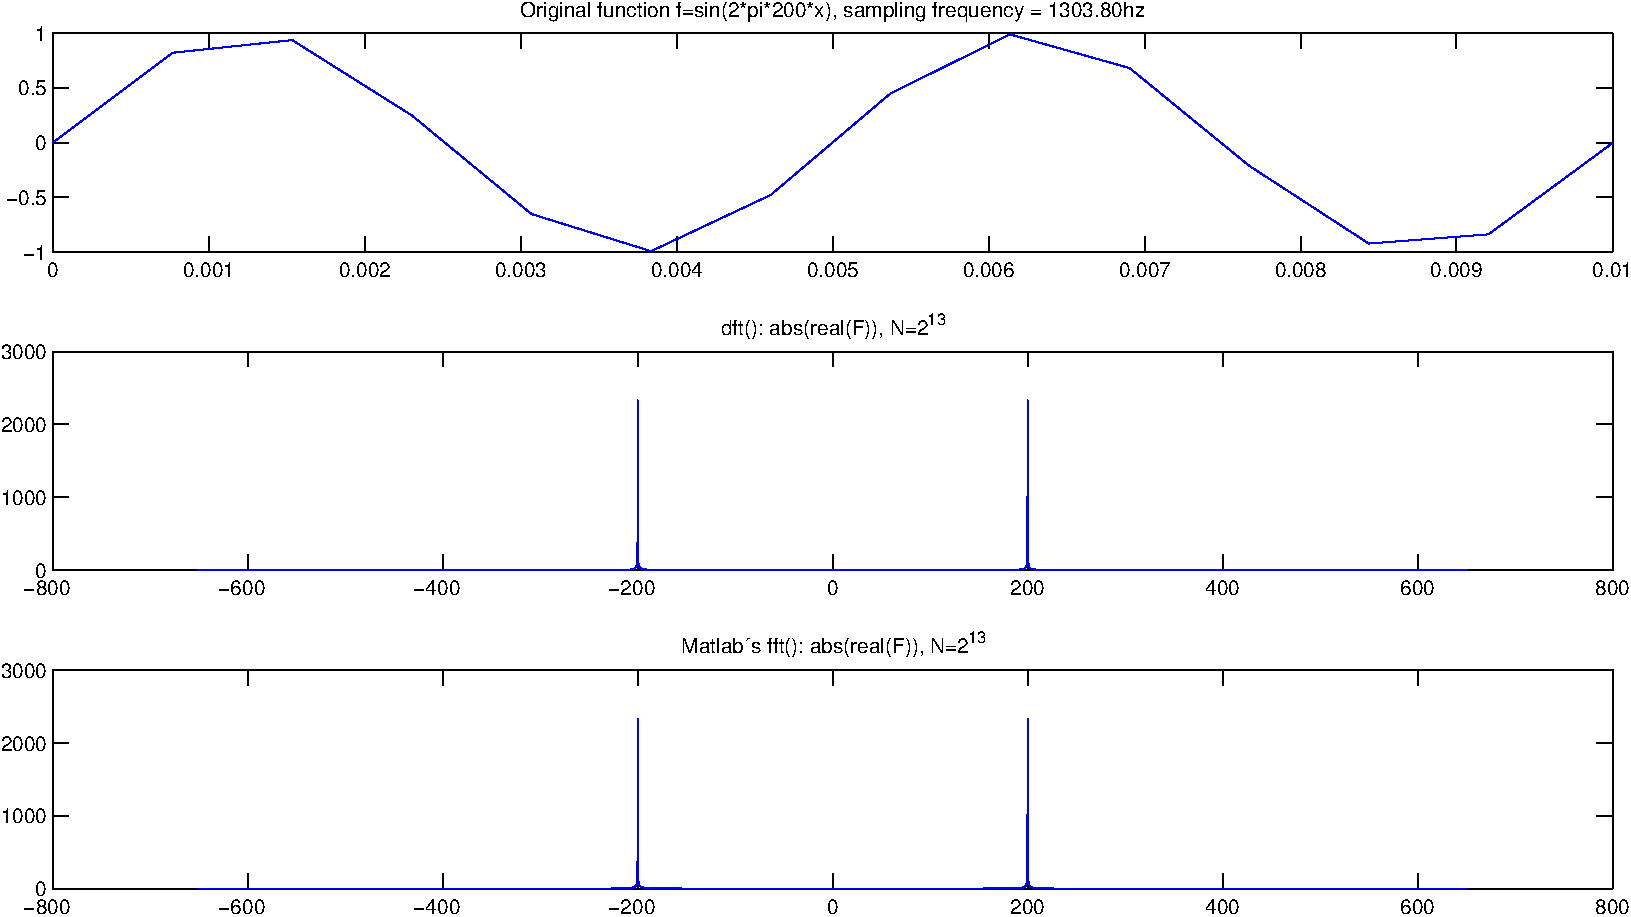
\includegraphics[height=200pt]{img/dft}
\end{myframe}

\begin{myframe}{DFT: Properties}

\vspace{-5px}

\begin{block}{\centering $\wn{j+N/2}=-\wn{j}$}
\begin{align*}
\wn{j+N/2} &= e^{ \frac{-2 \pi i (j+N/2)}{ N} } 
           = e^{ \frac{-2 \pi i j}{ N} + \frac{-2 \pi i (N/2)}{ N} }\\
           &= e^{ \frac{-2 \pi i j}{ N}} e^{-\pi i} 
            = -\wn{j}  
\end{align*}
\end{block}

\vspace{-5px}

\begin{block}{\centering $\wn{j+N}=\wn{j}$}
\begin{align*}
\wn{j+N} &= \wn{j+N/2+N/2}  = \wn{j}
\end{align*}
\end{block}

\vspace{-5px}

\begin{block}{\centering $F(k+N)=F(k)$}
\begin{align*}
F(k+N)&= \sumn x(n) \wn{(k+N)n} = \sumn x(n) \wn{kn} \wn{Nn}\\
 &=\dft = F(k)
\end{align*}
\end{block}
\end{myframe}



\begin{myframe}{FFT: Derivation (1) }
\centering
\begin{align*}
F_N (k)&= \dft = \sumnn x(2n) \wn{k (2n)} + \sumnn x(2n+1) \wn{k (2n+1)} \\
&= \sumnn x(2n) \wn{k 2 n} + \wn{k} \sumnn x(2n+1) \wn{k(2n)} \\
&= \sumnn x(2n) \wnn{kn} + \wn{k} \sumnn x(2n+1) \wnn{kn} \\
&= \fnneven (k) + \wn{k} \fnnodd (k) \qquad k=0,\dots,(N-1)
\end{align*}

\begin{block}{}
\centering
$\wn{k}$ are called \textit{twiddle factors}
\end{block}

\end{myframe}

\begin{myframe}{FFT: Derivation (2)}
\centering

\begin{block}{}
\centering
¿Value of $\fnneven(k)$ and $\fnnodd(k)$ if $k \geq N/2$?
\end{block}

Define $N_1=\{ 0,\dots,N/2-1 \}$ and $N_2=\{ N/2,\dots,N-1 \}$
%\small
\begin{align*}
\fn (k)&= \fnneven (k) + \wn{k} \fnnodd (k)\\
&= \begin{cases}
\fnneven (k) + \wn{k} \fnnodd (k) &\mbox{if } k \in N_1 \\
\fnneven (k) + \wn{k} \fnnodd (k) & \mbox{if } k \in N_2 \\
\end{cases}
\\  \text{If } k\geq N/2 &\rightarrow k=N/2+k'
\\ &= \begin{cases}
\fnneven (k) + \wn{k} \fnnodd (k) &\mbox{if } k \in N_1 \\
\fnneven (N/2+k') + \wn{N/2+k'} \fnnodd (N/2+k') & \mbox{if } k' \in N_1
\end{cases}
\\ &= \begin{cases}
\fnneven (k) + \wn{k} \fnnodd (k) & \mbox{if } k \in N_1 \\
\fnneven (k') - \wn{k'} \fnnodd (k') & \mbox{if } k' \in N_1
\end{cases}
\end{align*}

\end{myframe}

\begin{myframe}{FFT: Divide and conquer}
\centering
\begin{block}{Calculating $\fn(k)$ for all $k$}
\begin{enumerate}
\item Split $x(n)$ into $x_{odd}(n)$ and $x_{even}(n)$.
\item Calculate $\fnneven(k)$ and $\fnnodd(k)$ for all $k$
\item Calculate $\fn(k)$ for all $k$ as:
\begin{equation}
\fn (k) = \begin{cases}
\fnneven (k) + \wn{k} \fnnodd (k) & \mbox{if } k \in N_1 \\
\fnneven (k') - \wn{k'} \fnnodd (k') & \mbox{if } k' \in N_1, \; k=N/2+k'
\end{cases}
\end{equation}

\end{enumerate}
\end{block}
\end{myframe}

\begin{myframe}{FFT: Recursion splits}
\centering
\scalebox{0.75}{
    
\newcommand{\gridthing}[3]{ 




\pgfmathtruncatemacro\fend{#1/2-1} 

\foreach \s in {0,...,\fend}{
    \pgfmathtruncatemacro\xpos{#2-#1/2+\s*2} 
    \filldraw[fill=white] (\xpos,#3-1) rectangle (\xpos+1,#3);
}

\foreach \s in {0,...,\fend}{
    \pgfmathtruncatemacro\xpos{#2-#1/2+\s*2} 
    \filldraw[fill=gray!10] (\xpos+1,#3-1) rectangle (\xpos+2,#3);
}

}

\begin{tikzpicture}[level/.style={sibling distance=60mm/#1}]

\gridthing{8}{0}{9}

\draw[thick,->] (-3.5,8) -- (-4.5,6);
\draw[thick,->] (-1.5,8) -- (-3.5,6);
\draw[thick,->] (0.5,8) -- (-2.5,6);
\draw[thick,->] (2.5,8) -- (-1.5,6);

\draw[thick,->] (3.5,8) -- (4.5,6);
\draw[thick,->] (1.5,8) -- (3.5,6);
\draw[thick,->] (-0.5,8) -- (2.5,6);
\draw[thick,->] (-2.5,8) -- (1.5,6);

\gridthing{4}{-3}{6}
\gridthing{4}{3}{6}

\draw[thick,->] (-4.5,5) -- (-5.5,3);
\draw[thick,->] (-3.5,5) -- (-2.5,3);
\draw[thick,->] (-2.5,5) -- (-4.5,3);
\draw[thick,->] (-1.5,5) -- (-1.5,3);

\draw[thick,->] (4.5,5) -- (5.5,3);
\draw[thick,->] (3.5,5) -- (2.5,3);
\draw[thick,->] (2.5,5) -- (4.5,3);
\draw[thick,->] (1.5,5) -- (1.5,3);

\gridthing{2}{-5}{3}
\gridthing{2}{-2}{3}
\gridthing{2}{2}{3}
\gridthing{2}{5}{3}

\draw[thick,->] (-5.5,2) -- (-7,0);
\draw[thick,->] (-4.5,2) -- (-5,0);
\draw[thick,->] (-2.5,2) -- (-3,0);
\draw[thick,->] (-1.5,2) -- (-1,0);

\draw[thick,->] (5.5,2) -- (7,0);
\draw[thick,->] (4.5,2) -- (5,0);
\draw[thick,->] (2.5,2) -- (3,0);
\draw[thick,->] (1.5,2) -- (1,0);

\foreach \l in {0,...,7}{
    \filldraw[fill=white] (\l*2-7.5,0) rectangle (\l*2-6.5,-1);
}

%\foreach \l in {8,4,2}{
%    \pgfmathtruncatemacro\basexpos{\l} 
%    \pgfmathtruncatemacro\ypos{ln(\l)/ln(2)} 
%
%    \pgfmathtruncatemacro\items{4-\ypos} 
%    \foreach \b in {1,...,\items}{
%        \pgfmathtruncatemacro\xposs{\basexpos*(\b-1)} 
%        \gridthing{\basexpos}{\xposs}{\ypos*3}
%     }
%}



%\gridthing{4}{1}{3}


\end{tikzpicture}

} 
\end{myframe}

\begin{myframe}{FFT: Recursion tree}
\centering
\scalebox{0.85}{
    
\begin{tikzpicture}[level/.style={sibling distance=60mm/#1}]

\node [circle,draw] (z){$F_N$}
  child {node [circle,draw] (a) {$F_{\frac{N}{2}}$}
    child {node [circle,draw] (b) {$F_{\frac{N}{2^2}}$}
      child {node {$\vdots$}
        child {node [circle,draw] (d) {$F_{\frac{N}{2^k}}$}}
        child {node [circle,draw] (e) {$F_{\frac{N}{2^k}}$}}
      } 
      child {node {$\vdots$}}
    }
    child {node [circle,draw] (g) {$F_{\frac{N}{2^2}}$}
      child {node {$\vdots$}}
      child {node {$\vdots$}}
    }
  }
  child {node [circle,draw] (j) {$F_{\frac{N}{2}}$}
    child {node [circle,draw] (k) {$F_{\frac{N}{2^2}}$}
      child {node {$\vdots$}}
      child {node {$\vdots$}}
    }
    child {node [circle,draw] (l) {$F_{\frac{N}{2^2}}$}
        child {node {$\vdots$}}
        child {node (c){$\vdots$}
          child {node [circle,draw] (o) {$F_{\frac{N}{2^k}}$}}
          child {node [circle,draw] (p) {$F_{\frac{N}{2^k}}$}
          }
        }
    }
  }    
;
\path (o) -- (e) node (x) [midway] {$\cdots$};

\end{tikzpicture}

} 
\end{myframe}

\begin{myframe}{FFT: Implementation}
\centering
\lstinputlisting[basicstyle=\small\ttfamily]{code/facuft.m}
\end{myframe}

\begin{myframe}{FFT: Time complexity}
\centering
\lstinputlisting[basicstyle=\small\ttfamily]{code/facuft_time.m}
\end{myframe}

\begin{myframe}{FFT: Solving recurrence}
\centering

\only<1>{
\begin{block}{}
\begin{equation*}
T(n)= 
\begin{cases}
    D & \mbox{if} \; n=1 \\
    2T(\frac{n}{2})+Cn & \mbox{if} \; n > 1
\end{cases}
\end{equation*}
\end{block}
}

\only<2->{
\begin{block}{}
\begin{equation*}
T(n)= 
\begin{cases}
    1 & \mbox{if} \; n=1 \\
    2T(\frac{n}{2})+n & \mbox{if} \; n > 1
\end{cases}
\end{equation*}
\end{block}
}

\only<3>{
\begin{align*}
T(n)&= 2T(\frac{n}{2})+n = 2 (2T(\frac{n}{2^2})+\frac{n}{2})+n = 2^2 T(\frac{n}{2^2})+2\frac{n}{2}+n \\
&= 2^2 T(\frac{n}{2^2})+2n = \dots = 2^k T(\frac{n}{2^k})+kn \\
\mbox{If } \frac{n}{2^k}=1 &\rightarrow k = \log_2(n): \\
T(n)&= 2^{\log_2(n)} T(1) + \log_2(n) n = n+n \log_2(n) \in O(n \log(n))
\end{align*}
}

\end{myframe}

\begin{myframe}{FFT: Time complexity with recursion tree}
\centering
\scalebox{0.71}{
    
\begin{tikzpicture}[level/.style={sibling distance=60mm/#1}]
\node [circle,draw] (z){$n$}
  child {node [circle,draw] (a) {$\frac{n}{2}$}
    child {node [circle,draw] (b) {$\frac{n}{2^2}$}
      child {node {$\vdots$}
        child {node [circle,draw] (d) {$\frac{n}{2^k}$}}
        child {node [circle,draw] (e) {$\frac{n}{2^k}$}}
      } 
      child {node {$\vdots$}}
    }
    child {node [circle,draw] (g) {$\frac{n}{2^2}$}
      child {node {$\vdots$}}
      child {node {$\vdots$}}
    }
  }
  child {node [circle,draw] (j) {$\frac{n}{2}$}
    child {node [circle,draw] (k) {$\frac{n}{2^2}$}
      child {node {$\vdots$}}
      child {node {$\vdots$}}
    }
  child {node [circle,draw] (l) {$\frac{n}{2^2}$}
    child {node {$\vdots$}}
    child {node (c){$\vdots$}
      child {node [circle,draw] (o) {$\frac{n}{2^k}$}}
      child {node [circle,draw] (p) {$\frac{n}{2^k}$}
        child [grow=right] {node (q) {$=$} edge from parent[draw=none]
          child [grow=right] {node (q) {$O_{k = \lg n}(n)$} edge from parent[draw=none]
            child [grow=up] {node (r) {$\vdots$} edge from parent[draw=none]
              child [grow=up] {node (s) {$O_2(n)$} edge from parent[draw=none]
                child [grow=up] {node (t) {$O_1(n)$} edge from parent[draw=none]
                  child [grow=up] {node (u) {$O_0(n)$} edge from parent[draw=none]}
                }
              }
            }
            child [grow=down] {node (v) {$O(n \cdot \lg n)$}edge from parent[draw=none]}
          }
        }
      }
    }
  }
};
\path (a) -- (j) node [midway] {+};
\path (b) -- (g) node [midway] {+};
\path (k) -- (l) node [midway] {+};
\path (k) -- (g) node [midway] {+};
\path (d) -- (e) node [midway] {+};
\path (o) -- (p) node [midway] {+};
\path (o) -- (e) node (x) [midway] {$\cdots$}
  child [grow=down] {
    node (y) {$O\left(\displaystyle\sum_{i = 0}^k 2^i \cdot \frac{n}{2^i}\right)$}
    edge from parent[draw=none]
  };
\path (q) -- (r) node [midway] {+};
\path (s) -- (r) node [midway] {+};
\path (s) -- (t) node [midway] {+};
\path (s) -- (l) node [midway] {=};
\path (t) -- (u) node [midway] {+};
\path (z) -- (u) node [midway] {=};
\path (j) -- (t) node [midway] {=};
\path (y) -- (x) node [midway] {$\Downarrow$};
\path (v) -- (y)
  node (w) [midway] {$O\left(\displaystyle\sum_{i = 0}^k n\right) = O(k \cdot n)$};
\path (q) -- (v) node [midway] {=};
\path (e) -- (x) node [midway] {+};
\path (o) -- (x) node [midway] {+};
\path (y) -- (w) node [midway] {$=$};
\path (v) -- (w) node [midway] {$\Leftrightarrow$};
\path (r) -- (c) node [midway] {$\cdots$};
\end{tikzpicture}

} 
\end{myframe}

\begin{myframe}{FFT: Output}
\centering
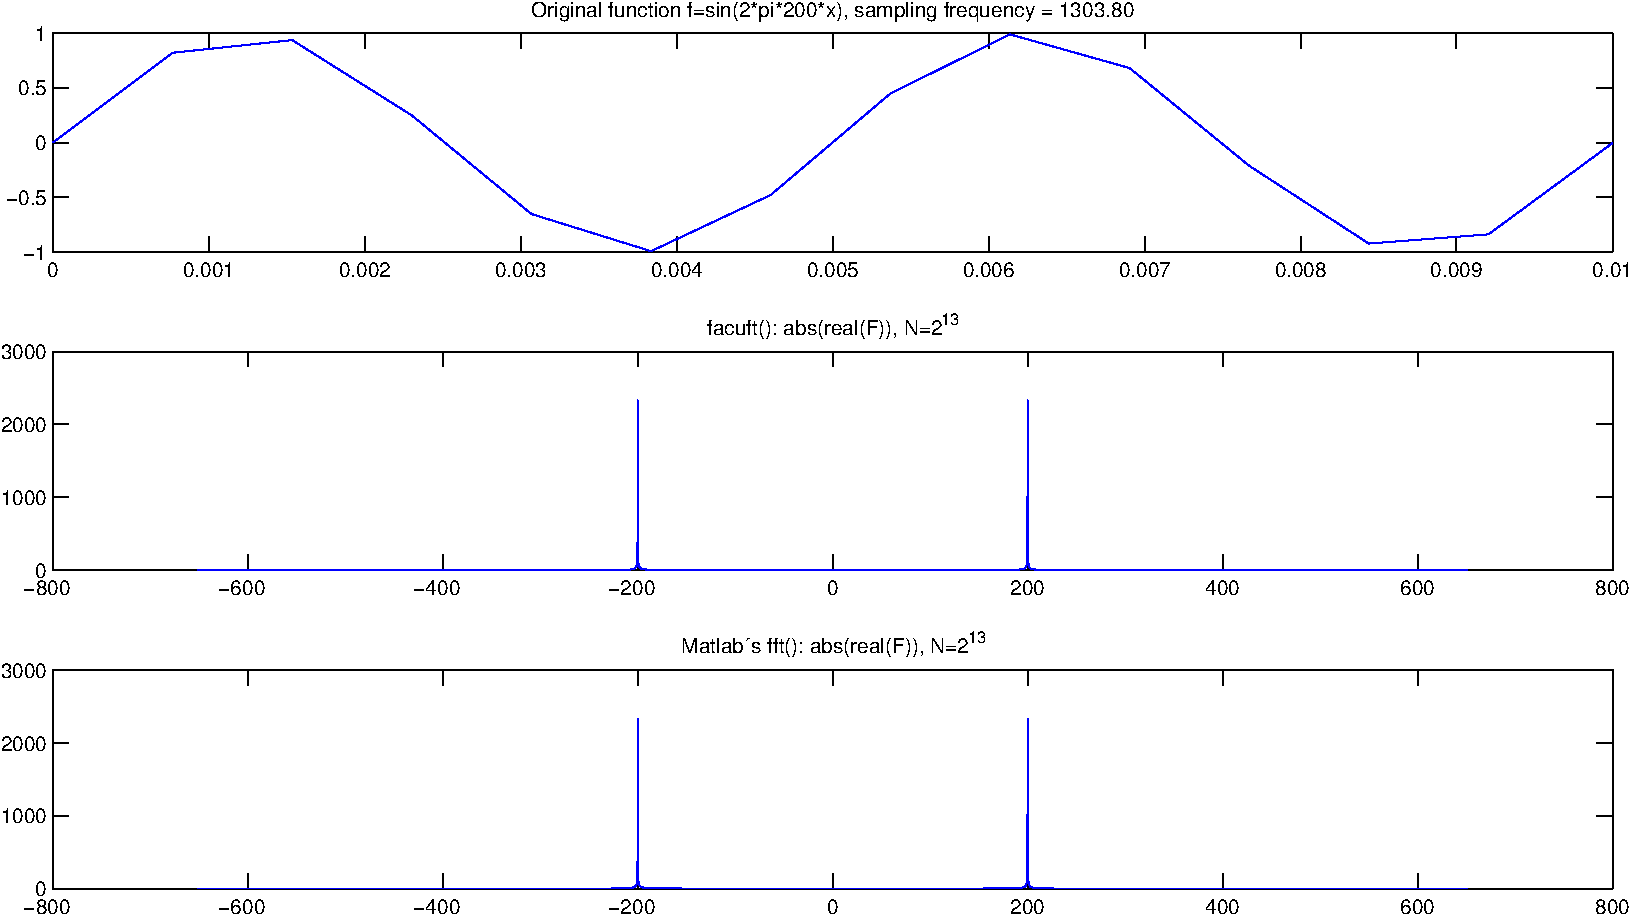
\includegraphics[height=200pt]{img/facuft}
\end{myframe}

\begin{myframe}{FFT: Empirical running time}
\centering
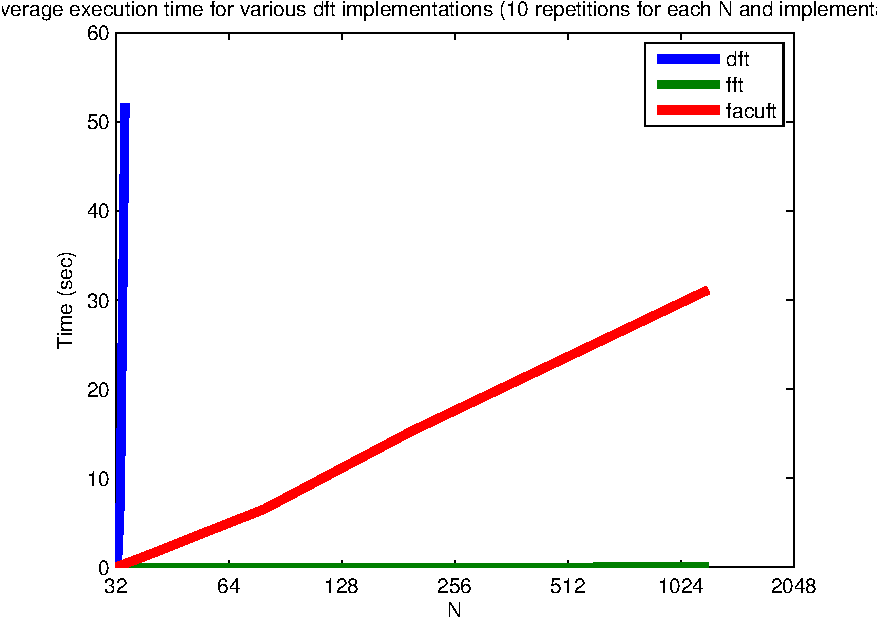
\includegraphics[height=200pt]{img/running_time}
\end{myframe}

\begin{myframe}{FFT: Implementation improvements}
\centering
\begin{itemize}
\item Recursion kills performance $\rightarrow$ bigger base cases
\item In every recursion call, split the input $x$ into $K$ subarrays instead of 2 (tree depth $= \log_K(n)$, \textit{fatter} trees) $\rightarrow$ Radix-m algorithms.
\item Recursion kills performance $\rightarrow$ iterative implementation
\item Calculate in-place (ie, no temporary arrays)
\item Avoid pure matlab (matlab's \texttt{fft} is written in C)
\item DFT's lower bound not known, but many results pointing to $DFT \in \Omega(n \log(n))$
\end{itemize}
\end{myframe}

\begin{myframe}{FFT: Bigger base case}
\centering
\lstinputlisting[basicstyle=\small\ttfamily]{code/facuft_basecase.m}
\end{myframe}

\begin{myframe}{FFT: Empirical running time}
\centering
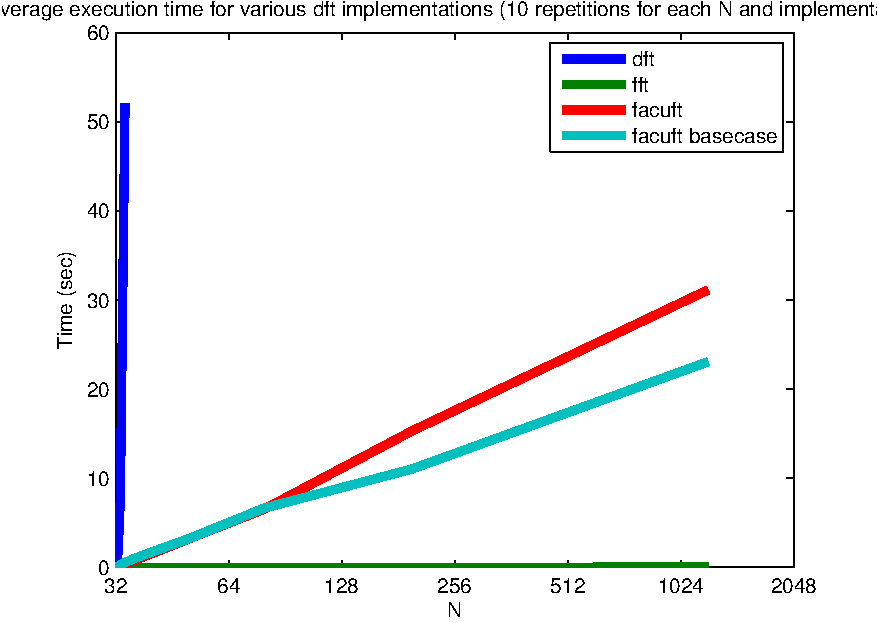
\includegraphics[height=200pt]{img/running_time_basecase}
\end{myframe}
\begin{myframe}{Matrix DFT}
\centering
\begin{align*}
\fn(k)&=\dft = (\wn{0k},\dots,\wn{(N-1)k}) \xv^T \\
\wvm &= \begin{bmatrix}
    \wn{0\times0}       & \wn{0\times1} & \dots & \wn{0\times(N-1)} \\
    \wn{1\times0}       & \wn{1\times1} &\dots & \wn{1\times(N-1)} \\
    \hdotsfor{4} \\
    \wn{(N-1)\times0}   & \wn{(N-1)\times1} &  \dots & \wn{(N-1)\times(N-1)}
\end{bmatrix}\\
(\wvm_{(k,n)} &=\wn{k \times n})\\
\fn(k) &= (\wvm \xv^T)_k 
\end{align*}
\begin{block}{}
\begin{equation*}
\fnv \xv = \wvm \xv^T 
\end{equation*}
\end{block}

\end{myframe}

\begin{myframe}{FFT Review}
\centering

\begin{block}{Calculating $\fn(k)$ for all $k$}
\begin{enumerate}
\item Split $x(n)$ into $x_{odd}(n)$ and $x_{even}(n)$.
\item Calculate $\fnneven(k)$ and $\fnnodd(k)$ for all $k$
\item Calculate $\fn(k)$ for all $k$ as:
\begin{equation}
\fn (k) = \begin{cases}
\fnneven (k) + \wn{k} \fnnodd (k) & \mbox{if } k=0,\dots,N/2-1 \\
\fnneven (k') - \wn{k'} \fnnodd (k') & \mbox{if } k=N/2,\dots,N-1 
\end{cases}
\end{equation}
($k=k'+N/2$)
\end{enumerate}
\end{block}

\begin{block}{Factorization}
Operations \textbf{1}, \textbf{2} and \textbf{3} can be expressed as a matrix too.
\end{block}

\end{myframe}


\begin{myframe}{Matrix FFT: Factorization}
\centering

\begin{align*}
\fnv \xv &=  
\begin{bmatrix}
\ve{I} &  \ve{D_N} \\
\ve{I} &  \ve{-D_N}
\end{bmatrix}  
\begin{bmatrix}
\fnnv & 0 \\
0 & \fnnv 
\end{bmatrix}  
\begin{bmatrix}
1 & 0 & 0 & 0 & \dots  \\
0 & 0 & 1 & 0 & \dots \\
\vdots & \vdots & \vdots &  \vdots &  \\
0 & 1 & 0 & 0 &  \dots  \\
0 & 0 & 0 & 1 & \dots \\
\vdots & \vdots & \vdots & \vdots & 
\end{bmatrix}  \xv
\\
&=  
\cmv_N
\begin{bmatrix}
\fnnv & 0 \\
0 & \fnnv
\end{bmatrix}  
\pmv_N
\xv
\end{align*}

\begin{block}{D diagonal, with twiddle factors}
\begin{equation}
\ve{D_{N(i,i)}}= \wn{i}, \qquad i=0,\dots, N-1
\end{equation}
\end{block}

\end{myframe}

\begin{myframe}{Matrix FFT: Factorization}
\centering

\begin{align*}
\fnv \xv &=  
\cmv_N
\cmv_{N/2}
\begin{bmatrix}
\fnnnv & 0 & 0 & 0\\
0 & \fnnnv & 0 & 0 \\
0 & 0 & \fnnnv & 0  \\
0 & 0 & 0 & \fnnnv\\
\end{bmatrix}  
\pmv_{N/2}
\pmv_N \xv\\
&=
\cmv_N
\cmv_{N/2}
\cmv_{N/2^2}
\dots
\cmv_{1}
\ve{I}
\pmv_{1}
\dots
\pmv_{N/2^2}
\pmv_{N/2}
\pmv_N \xv\\
&= 
\cmv_N
\cmv_{N/2}
\cmv_{N/2^2}
\dots
\cmv_{1}
\pmv_{1}
\dots
\pmv_{N/2^2}
\pmv_{N/2}
\pmv_N \xv\\
\end{align*}

\end{myframe}
\begin{myframe}{Matrix FFT: Iterative}
\centering

\begin{block}{Calculating $\fn(k)$}
\begin{enumerate}
\item Apply $\log_2(n)$ permutations $\pmi$ to $\xv$ to obtain $\xv'$
\item Apply $\log_2(n)$ combination operations $\cmi$ to $\xv'$ to obtain $\fn(\xv)$
\end{enumerate}
\end{block}


\begin{block}{Running time}
\begin{itemize}
\item Even though each permutation and combination operation is represented by an N-by-N matrix, it can be applied in $O(n)$ time
\item Each item above is therefore $O(n \log(n))$
\item Total running time is still $O(n \log(n))$
\end{itemize}
\end{block}

\end{myframe}

\begin{myframe}{Iterative FFT: Implementation}
\centering
\lstinputlisting[basicstyle=\small\ttfamily]{code/facuft_iterative.m}
\end{myframe}

\begin{myframe}{Iterative FFT: Output}
\centering
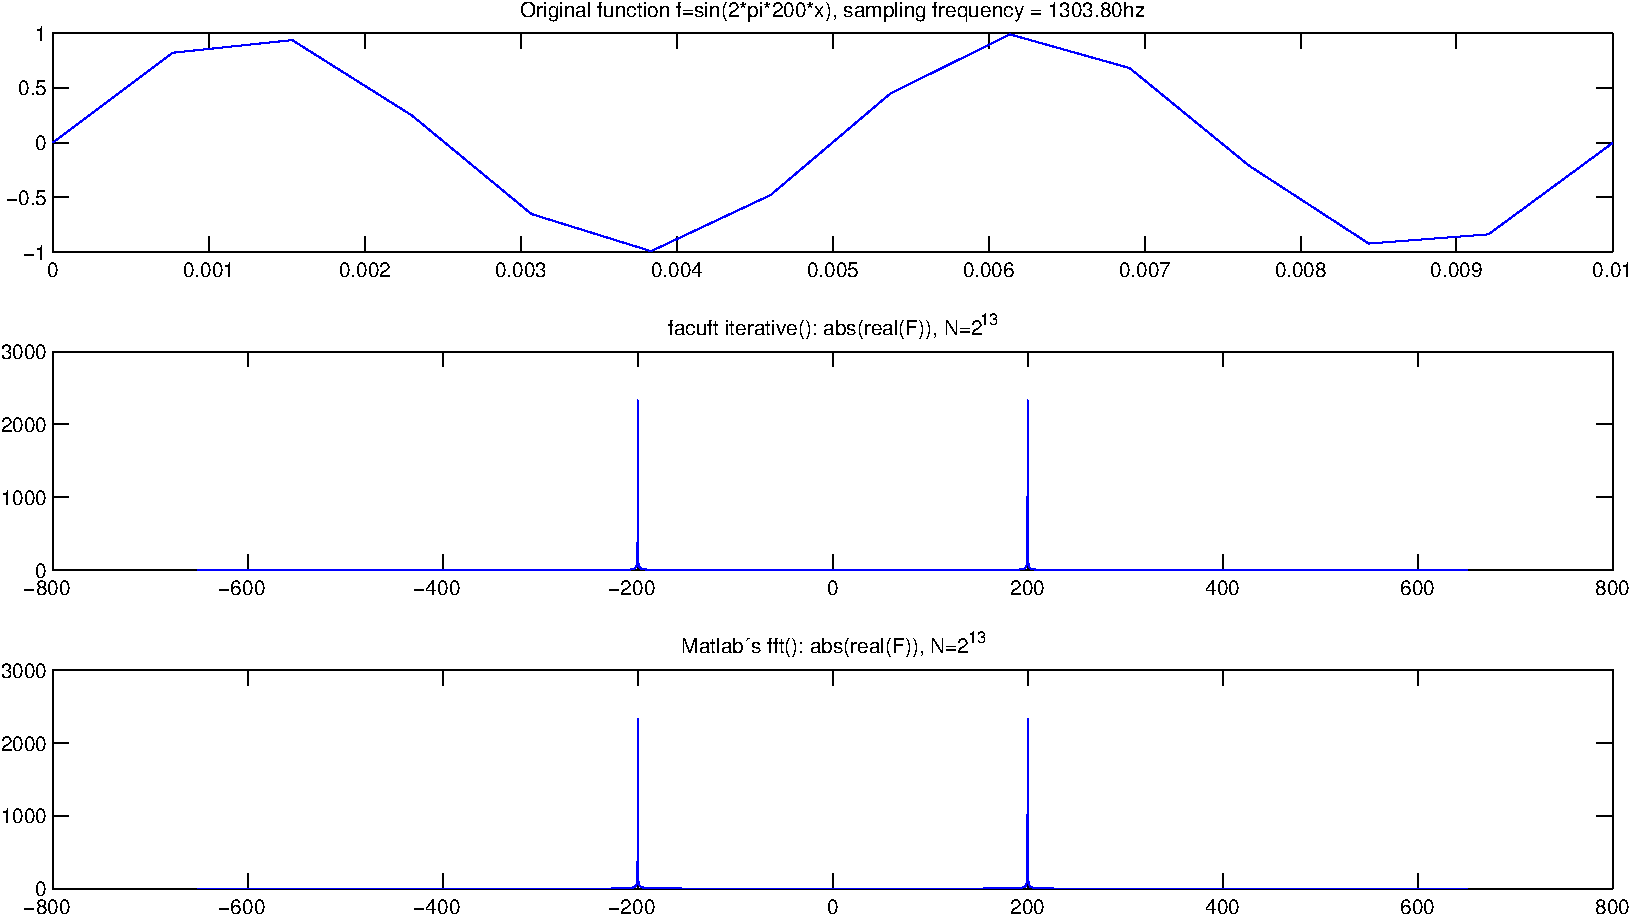
\includegraphics[height=200pt]{img/facuft_iterative}
\end{myframe}

\begin{myframe}{Iterative FFT: Empirical running time}
\centering
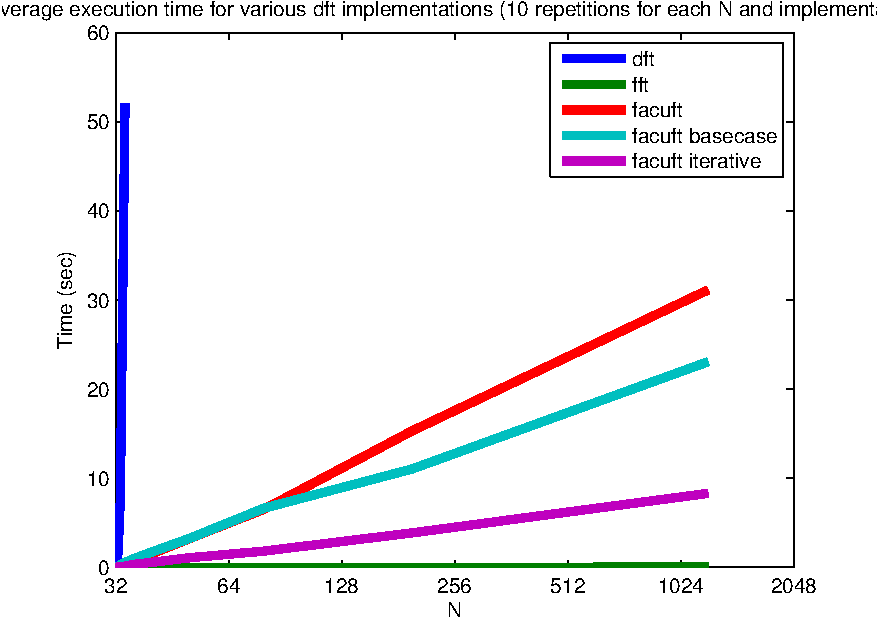
\includegraphics[height=200pt]{img/running_time_iterative}
\end{myframe}

\end{document}
